\chapter{Public services in Smart Cities}
\label{intro} 


\abstract{
\\ (1 or 2 lines): Give a context of your project
\\(1 line): what is the problem?
\\(2 lines): how are you solving it?
\\(1 or 2): what are the results/conclusions
}

\section{Introduction}
\label{sec:1}


\section{Related works}
\label{sec:2}

The research group BLABLA \cite{cheng2015building} did a similar work....using MQTT as it is shown in Figure \ref{fig:1}.
\begin{figure}
\sidecaption
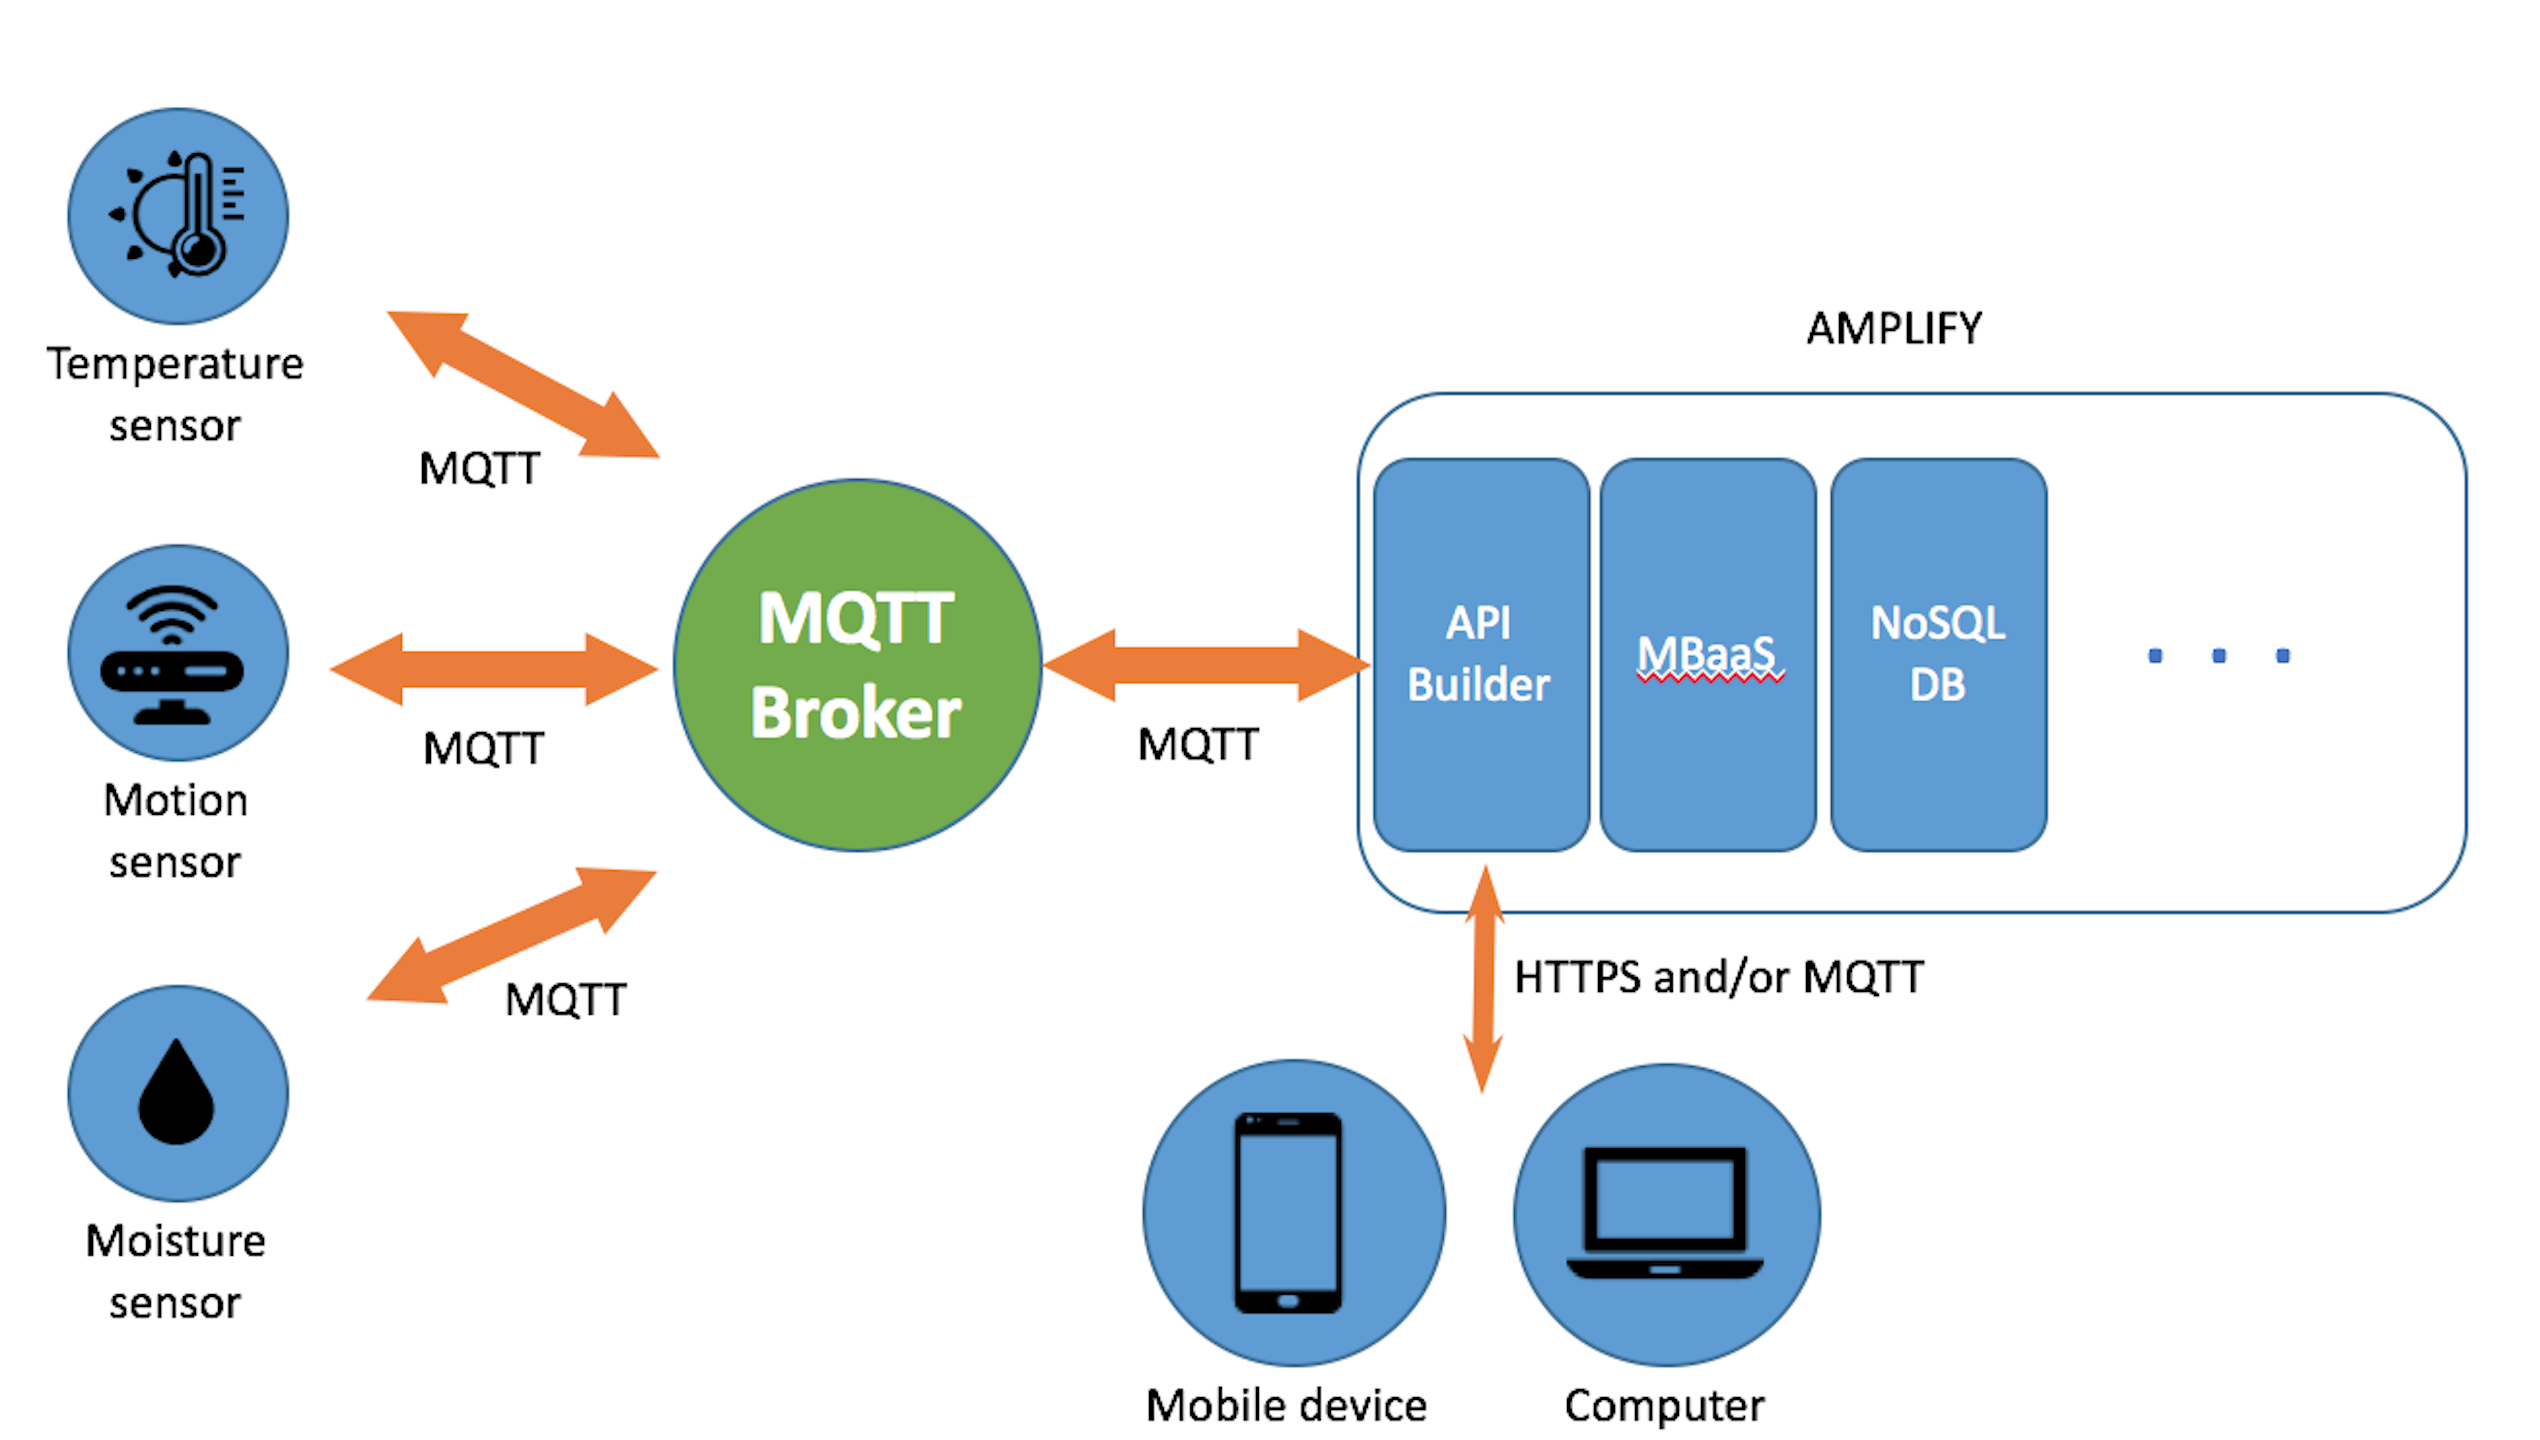
\includegraphics[scale=.09]{images/figure.png}
\caption{this is a picture}
\label{fig:1}
\end{figure}


\section{Your proposal (Concept)}
\label{sec:3}
   What is your project?
\\ requirements table
\\ Add a picture explaining how it works (concept)
\\ Diagrams
\\

\section{Implementation of your proposal}
\label{sec:4}
   if you have class diagram
\\ or an image that show parts of your system
\\ screenshots of part of your code
\\ explain the main parts of the code
\\ make a relation between the functionalities of the system and the requirements
\\ like: this part of the code does that which is described in the requirement FR1.

\section{Results}
\label{sec:5}
   show what is working
\\ which requirements are not implemented?
\\ what could you have done in a different way?

\section{Conclusion}
\label{sec:5}
...
\\ future work